\documentclass{beamer}


\usepackage[utf8]{inputenc}
\usepackage{amsmath}
\usepackage{amsfonts}
\usepackage{amssymb}
\usepackage{graphicx}
\usepackage{ragged2e}  % `\justifying` text
\usepackage{booktabs}  % Tables
\usepackage{tabularx}
\usepackage{tikz}      % Diagrams
\usetikzlibrary{calc, shapes, backgrounds}
\usepackage{amsmath}
\usepackage{amssymb}
\usepackage{dsfont}
\usepackage{url}       % `\url
\usepackage{listings}  % Code listings
\usepackage[T1]{fontenc}


\usepackage{theme/beamerthemehbrs}

\author[MAS]{Hassan Umari}
\title{Introduction to ROS}
\subtitle{Foundation Course}
\institute[HBRS]{Hochschule Bonn-Rhein-Sieg}
\date{\today}
\subject{ROS workshop}

% \thirdpartylogo{path/to/your/image}


\begin{document}
{
\begin{frame}
\titlepage
\end{frame}
}


\section{What is ROS?}


\subsection{What ROS is}
\begin{frame}{What ROS is}
\framesubtitle{Robot Operating System}
    \begin{itemize}
        \item Short for: Robot Operating System.
        \item A collection of libraries and tools.
        \item It helps software developers create robot
        applications. 
    \end{itemize}
\end{frame}



\begin{frame}[plain]{}
    \centering
    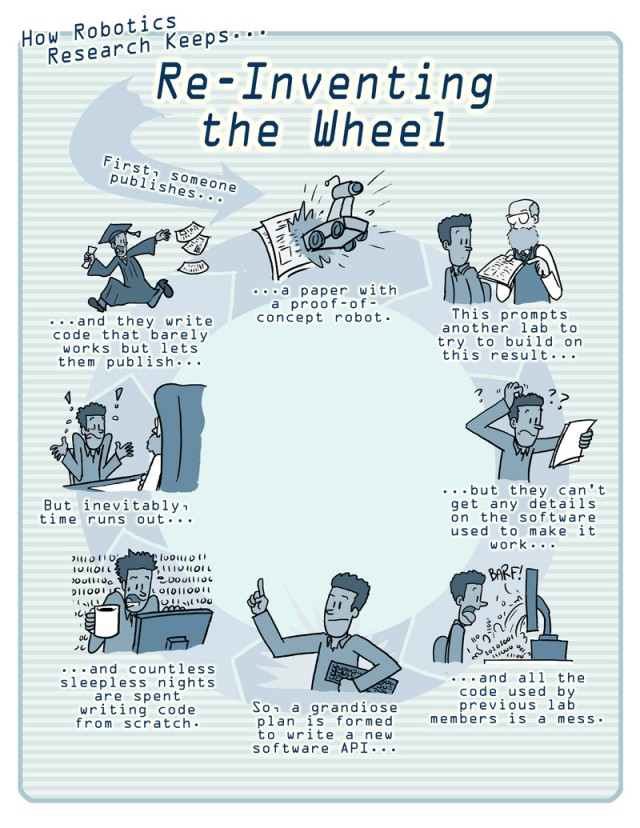
\includegraphics[width=.66\linewidth]{figures/stop_reinventing_theWheel.jpg}
    
\tiny{http://www.willowgarage.com/blog/2010/04/27/reinventing-wheel}
\end{frame}


\begin{frame}{What ROS is}
    \framesubtitle{Robot Operating System}
    \begin{itemize}
        \item A way to standardize writing software for robots.
        \item It enhances {\huge code reusability} 
\includegraphics[scale=0.02]{figures/recycling.png}.
        \item ROS is open-source 
\includegraphics[scale=0.09]{figures/openSource.png}.
        \item It is a meta-operating system.
        \item ROS can be installed on Ubuntu and Debian (so it’s currently supported on Linux only). 
    \end{itemize}
\end{frame}


\subsection{What ROS is NOT}




\end{document}
